\documentclass[12pt]{article}
\usepackage{uwyo_report} 
\usepackage{textcomp}
\usepackage{titlesec}
\usepackage{listings}
\titleformat{\section}[block]{\bfseries\filcenter}{}{1em}{}
\titleformat{\subsection}[hang]{\bfseries}{}{1em}{}
\hyphenation{con-sti-tu-tion-al}

\begin{document}

\title{EE 4830 \\
Final Paper \\}

\author{Stephen Boyer \\
Electrical and Computer Engineering Department \\
College of Engineering \\
University of Wyoming \\
Laramie, WY 82071 \\
\texttt{sboyer3@uwyo.edu}}
\date{}
\maketitle

\begin{abstract}
This project consists of interfacing an application running on a Google Android device with two external devices to implement an infrared television controller. The first of the two external devices is a \emph{hub} device to connect to the user's existing wireless fidelity (WiFi) network. It has a radio frequency transmitter enabling it to communicate with the second external device, a battery-powered \emph{child} device. This device contains an IR receiver and transmitter pair for learning IR codes from a television remote and sending them to a television, respectively.

This project was chosen mainly to reduce the number of devices a user must keep track of. Once the remote codes are learned by the system, a dedicated television remote is redundant. Since, unlike with infrared communication, radio frequency and WiFi communication do not require line of sight, users are not required to point anything at the television or even be in the same room. Conveniently, many people already own a phone or tablet running the Android operating system. With this system, an application could easily be developed to work with Apple's iOS or essentially any platform allowed to run third-party programs.  
\\
\\
\noindent \textbf{Keywords:} Arduino, Android, Raspberry Pi, infrared, television, remote, LED, RF
\end{abstract}

\section*{Overview}
This television control system was completed over the past year. From the start of the project, the goal was to make an adaptable system for controlling one or more televisions using an infrared (IR) light-emitting diode (LED). This works similarly to how a normal television remote works. Up to three televisions are supported by the Android application although enough equipment was only made for one. In order to control more televisions, a user would only need more \emph{child} devices as the \emph{hub} can communicate with more than one. 

The system functions by sending commands over wireless fidelity (WiFi) to the \emph{hub} device which forwards them to the \emph{child} device over radio frequency (RF) communication. A special feature of this system is that of the \emph{child} device to ``learn" IR remote codes. This means that any brand or model of television is supported as long as its remote uses IR. 

Included in this paper are background, technical, testing, and packaging sections. These are followed by other considerations and lessons learned. Also included are a schedule, parts list, circuit diagram, construction diagram, structure and activity diagrams, and code. 

\section*{Background}
 Communication between devices is the most important factor of this project. The first aspect of this is communication between the Android application and the \emph{hub} device. WiFi was chosen for this as it provides good range and is already used in homes everywhere. The downside is that it uses a large amount of power which is why the \emph{hub} device runs off of a wall adapter instead of batteries. The second aspect of the communication problem is between the \emph{hub} and \emph{child} devices. RF communication at a frequency of 315 megahertz (MHz) was chosen for this for its relative simplicity and low power requirements. The power requirements allow the \emph{child} to run off of battery power. The final type of communication used is infrared between the \emph{child} and television being controlled. Most TVs today use infrared light with a wavelength of 950 nanometers for control so this was the only option.  
 
Google Android is a Linux-based smart phone operating system (OS) originally released in 2009. In this project, Android 4.4 or ``KitKat" is used. The application will run on any newer version as well. Android applications are programmed and designed using the Android Software Development Kit (SDK) and elements of the Java Development Kit (JDK). Java is the predominant programming language used here. The Android SDK defines the base requirements an application must have. For starters, a \texttt{MainActivity.java} file is used to define and implement the main Activity for an application. In Android, Activities are used as windows in which user interaction takes place. An \texttt{AndroidManifest.xml} file is required for defining the Activities in use in the application, any permissions the application requires from the Operating System, and any Intents used. The only permission used here is for Internet access. Although the Internet is not actually accessed, WiFi access requires this permission regardless.  In Android, Intents are used for opening Activities. Here, Intents are used for opening the application from the launcher in Android as well as opening an Activity where settings are displayed. A \texttt{build.gradle} file defines the version of Android an application is being compiled against. Here, SDK version 19 is used. This represents Android 4.4. According to the Android Open Source Project, 47\% of Android devices use this version or above \cite{aosp}.

\section*{Technical Project Description}
This project included three distinct parts: an Android application running on a smartphone, a \emph{hub} device for relaying commands, and a \emph{child} device for receiving commands and forwarding them to a television. Together, these parts make up a system for controlling a television easily.

Other than powering on the \emph{hub} and \emph{child} devices, user interaction is done exclusively with the Android application. Once the user presses a virtual button, a signal is sent to the \emph{hub} device over WiFi. The device in question is a Raspberry Pi B+ with a Universal Serial Bus (USB) WiFi adapter. It also has a small printed circuit board (PCB) with a RF transmitter attached. The \emph{hub} responds by sending a corresponding signal to the \emph{child} device via its RF transmitter. This signal is received by the RF receiver on the \emph{child} device, an Arduino UNO R3. Depending on the command, the \emph{child} turns on its IR receiver to wait for a signal from a remote control, turns on its IR LED and sends a signal to a television, or erases all codes from its memory.  

\subsection*{Android Application}
The first part of the system is the Android application running on a smartphone with Android 4.4 or above. As is typical of Android applications, this is programmed in the Java programming language. The Extensible Markup Language (XML) is utilized for defining the build configuration, interface, preferences, and some variables. 

The interface of the application is a grid of buttons for the various functions of a standard remote control. In addition to buttons numbered 0-9 for channels, there are buttons for power, input source, volume up and down, channel up and down, and mute. There is also a button labeled ``Favorites", the pressing of which causes a list of favorite channels to pop up. In the upper right corner of the application is a button labeled ``Settings" which takes the user to a page where preferences such as Internet Protocol (IP) address, port number, password, and username needed to communicate with the \emph{hub} device. These settings should not have to be changed for this project, but it is a good idea to make them editable for users. The last two settings are ``Reset Recorded Buttons" and ``Set Favorite Channel". ``Reset Recorded Buttons" causes the app to send a signal to the \emph{hub} to cause the \emph{child} to erase all stored IR codes. There are three horizontal bars in the upper left corner of the application. When pressed, a menu slides out from the left and allows the user to change to other TVs or \emph{child} devices. The final button in the interface is a switch at the bottom. When toggled by pressing, this switch changes the mode of operation of the app from ``Button Mode", for sending recorded button presses to the \emph{hub}, to ``Record Mode" for sending a signal to the \emph{hub} representing a command to record along with the button pressed.

The commands being sent from the application are Hypertext Transfer Protocol (HTTP) POST requests. An HTTP server running on the Raspberry Pi-based \emph{hub} device listens for these requests and acts on them. The request takes the form of a URL as follows:
\begin{quote}
http://[IP Address of Hub]:[Server Port]/macros/[Command Type]/[Button Number]. 
\end{quote}
JSON (JavaScript Object Notation) is used for sending requests. The password and username are sent to the \emph{hub} using a JSONParser which is used along with the URL above to create a JSONObject. At the creation of this object, the command itself is sent out over the Android device's WiFi connection. Because of requirements in Android, this process is completed in a thread separate from the rest of the application. This thread starts when a button is pressed and stops after a command is sent.       
 
 
 \subsection*{Hub Device}
The second part of the system is the \emph{hub}. It is based on a Raspberry Pi B+ running Raspbian OS. Like Android, this operating system is based on Linux. To create the listening server, a library called WebIOPi was used. This framework is developed by Eric Ptak and released under the Apache license \cite{webiopi}. WebIOPi is developed in Java with a Python-based Application Program Interface (API). It simplifies the creation of an HTTP server capable of listening for of the POST from from another device. In this case, it listens for commands from the Android app. The WebIOPi library is used through the running of a Python script (see Listing \ref{code_gpio} in the Code section of the Appendix) that starts a server on the Raspberry Pi's IP address with a port number defined in a configuration file located on its Secure Digital (SD) card at \texttt{/etc/config/webiopi}. The default is port $8000$. In this same file, the username and password for the server can be modified. Naturally, to function correctly, the settings configured here must match those in the settings section of the Android application.
 
When a command is received, the corresponding function is called. For instance, a command of the form 
 \begin{quote}
 http://10.10.0.1:8000/macros/sendButton/1
 \end{quote}
 will be received by the hub at $10.10.0.1$ via port $8000$. The \texttt{sendButton(button)} function in the Python script will be called with an argument 1 for \texttt{button}. The function \texttt{sendButton} blinks the yellow status LED once before sending a shortened representative command to the \emph{child} via RF. The shortened command takes the form 
 \begin{quote}
[Child Number][Command Type][Button Number].
 \end{quote}
In the above example, Child Number would be 0 for the one and only \emph{child} created in the scope of this project. This field is only present so that it is possible to add more \emph{child} devices if the user desires them. If this number does not match the number of the \emph{child} receiving it, the \emph{child} will ignore the command. For command type, there are three possible values: $0$ for \texttt{sendButton}, $1$ for \texttt{sendRecord}, and $2$ for \texttt{resetChild}. \texttt{Button Number} is simply an integer representing the number the button is assigned in the Android application. The numbers are only used for keeping track of what button was pressed and are meaningless otherwise. For the current application with 17 total buttons, the numbers range from 0 to 16.

The final part of the \emph{hub}'s PCB is an antenna connected to the antenna pin of the RF transmitter. It is a simple piece of wire standing vertically. Its length is approximately $23.8 cm$, which is equivalent to a quarter of the wavelength of a 315 MHz signal. This is according to the formula for wavelength, 
\[\gamma=\frac{v}{f}\]
\cite{wavelength}, where $\gamma$ is wavelentch, $v$ is velocity, and $f$ is frequency. In this case, $v=299,792,458 \frac{meters}{second}$, or the speed of light. For a frequency of 315 MHz, $f=315,000,000$. One quarter of this value is found to be $23.8 cm$.
 
 \subsection*{Child Device}
 
 The final device is the one responsible for receiving commands from the \emph{hub} and is known as the \emph{child}. It is based on an Arduino Uno R3, surface-mount device (SMD) edition. In this project's original description, the \emph{child} was to be based on a Texas Instruments MSP430. However, due to the small Random Access Memory (RAM) size of this device, this was deemed impossible. Texas Instruments does not make a device in this line with more RAM. The Arduino Uno R3's 2 kilobyte RAM size is four times that of the MSP430 and is more than adequate. 
 
 The \emph{child} has three roles: recording IR remote codes, storing them in its non-volatile Electrically Erasable Programmable Read-Only Memory (EEPROM), and playing them back when necessary. It has an IR receiver module for recording messages and an IR LED for playing them back. There are two other LEDs, one red and one yellow. Finally, there is a 315 MHz RF receiver. The \emph{child} and components are powered together using six AA batteries in a holder. This provides the approximately nine volts required by the Arduino. Voltage is stepped down to five volts for the remaining components with two voltage regulators. Everything is turned on and off with a slider switch mounted on the PCB with all of the other components external to the Arduino.
 
 Receiving codes from the \emph{hub} is done via the RF receiver. A library known as VirtualWire \cite{virtualwire} is used to help with this. It runs on the \emph{hub} as well as the \emph{child}. As stated previously, these commands are received in the form
 \begin{quote}
 [Child Number][Command Type][Button Number].
 \end{quote}
Whereas these codes are sent from the \emph{hub} as standard American Standard Code for Information Interchange (ASCII) characters, they are received by the \emph{child} as hexadecimal representations of those ASCII characters. For instance, the code ``0" for the Child Number translates to $0x30$ in hexadecimal. This value is compared to a constant \texttt{CHILD\_ID} to determine if the code is meant for the \emph{child} receiving it. If not, the \emph{child} ignores the command. However, if the code does match, the next step is to determine the command. This is done by comparing the second character in the command to $0$ ($0x30$) for \texttt{sendButton}, $1$ ($0x31$) for \texttt{sendRecord}, and $2$ ($0x32$) for \texttt{sendReset}. Finally, if \texttt{Button Number} contains two digits, the third and fourth characters are combined to form the number used by the \emph{child}. This is needed because the characters are sent serially. Otherwise, the third character is used by itself.    
 
 When the command is \texttt{sendRecord}, the IR receiver is turned on. It is a Vishay Electronics TSOP38238, which is designed to demodulate 38 kilohertz (kHz) IR signals. The fact that it demodulates signals means that it can be connected directly to a microcontroller. Signals leaving the IR receiver enter a digital input pin on the Arduino. Because of the demodulation, the codes comes in as digital pulses.  From here, a library is used to simplify recording IR remote codes. It also simplifies playing them back later on. This library is known as IRremote and is written by Ken Sheriff \cite{irremote}. The library also helps in storing IR codes. In this case, EEPROM is used to store codes as it is non-volatile and good for long-term storage. After being processed using the library, the codes are represented by alternating marks and spaces which are equivalent to time high and time low, respectively. These times are measured in microseconds.

 For the command \texttt{sendButton}, the IR LED is turned on. This LED has a wavelength of 950 nanometers just like television remotes. Using pulse-width modulation (PWM), the LED turns on and off for the time for the number of microseconds defined by marks and spaces, respectively. Humans cannot see infrared light due to its long wavelength. Any light with a wavelength above approximately 700 nanometers is invisible to humans \cite{nasa}. As such, there is no way to see the 950 nanometer IR LED light up with the naked eye. To counteract this problem, a red LED runs in parallel with the IR LED to give visible feedback. Both of these LEDs utilize a 2N3904 n-channel biased junction transistor in a common-emitter amplifier arrangement to provide more current and therefore light than the Arduino Uno could manage otherwise. They are connected one of the Arduino's PWM pins. 
 
 The final command that can be received is \texttt{sendReset}. This causes the Arduino to erase all stored IR codes. It is only sent when ``Reset Recorded Buttons" is pressed in the ``Settings" screen of the Android app.   
 
 A yellow LED is used to show the status of the child. It is connected to one of the Arduino's digital out pins. This LED is turned on once the Arduino has finished booting. It flashes a certain number of times when each type of command is received; once for \texttt{sendRecord}, twice for \texttt{sendButton}, three times for \texttt{sendReset}, and four when it does not recognize a command. After blinking, the LED remains turned on steadily to show that the \emph{child} is turned on. 
 
 The original specifications for this project included a battery life of one month for the \emph{child}. Of course, these specifications were for a \emph{child} built using a TI MSP430. The MSP430 was originally chosen for its low power consumption. An Arduino does not share in this quality which led to a resulting battery life of around 6 days instead of 30. 
 
\section*{Testing}
This system was tested by using it as a normal user would. To begin, a user would install the application on his/her Android device and open it. Then he/she would open the settings section of the application and adjust the ``Username", ``Password", ``IP Address", and ``Port Number" sections for his/her \emph{hub} device. The default settings in the application would usually be adequate. 

The next step would be to begin ``teaching" the hub device remote codes. This is done by toggling the ``Record Mode" switch on the bottom of the main application screen to the ``On" position. Then, the user would press a button (e.g. ``Power") on the screen and wait for the yellow status LED to light up on the ``child" device. This signals that the device is waiting for an input on the infrared sensor representing a remote code. The user would press the button corresponding to the button pressed in the application (e.g. ``Power") on the TV's remote control while pointing it toward the \emph{child}. Then, the status LED would turn off, signifying a recorded remote code. This ``teaching" process would be repeated with different buttons of the remote application until the user is satisfied. 

The final step of testing would be to ensure the recorded remote codes work as expected. This would be done by toggling the ``Record Mode" switch on the bottom of the main application screen to the ``Off" position for playback of codes. Then, several buttons would need to be pressed to see if the TV performed the correct functions. If this test is passed, the system is working as specified. Testing performed on April 21, 2015 confirmed this was the case.

Other tests included keeping the \emph{hub} and \emph{child} turned on for five days continuously to simulate real-world operating conditions. The same test as above was run to ensure everything continued to function. This test was passed as well. 

\section*{Packaging}
 Packaging was taken care of using two clear, plastic boxes purchased from Amazon. Plastic was used instead of aluminum or another metal so that RF signals would be uninhibited. The plastic is clear for the \emph{child} so that IR signals will travel through and so that the user can see the red and yellow status LEDs. The plastic on the \emph{hub} is clear to match the \emph{child}. In total, this packaging costed \$18.92. The container for the \emph{hub} device is a small box designed for a Raspberry Pi. A small board with the red status LED and RF transmitter sits glued atop. For the \emph{child}, a box large enough to hold the Arduino, PCB, and battery pack was used.

\section*{Other Considerations}
\subsection*{Project Cost}
The total cost of this project turned out to be $\$135.43$. See the table under Parts List in the Appendix for a breakdown of parts and their prices. A wireless router is not included. Originally, this was under the assumption that most people in the United States already own wireless routers. As it turns out, the Raspberry Pi can also be configured to run as a wireless router. This option was used when testing and demonstrating. The price of the Android device was not included either. Similar to a wireless router, this was done under the assumption that most people in United States have smartphones. Not all of them run Android, but those running iOS or Windows Phone would only need an application to be made for them. A television was not included either for the same reasons. Therefore, for these reasons and in order to save approximately $\$500$, a wireless router, smartphone, and television were not included in the price. 

\subsection*{Ethical and Social Considerations}
There are two potential ethical and social considerations with a device like this. The first comes with any Internet-enabled device: security. Knowingly designing a product that allows users to get hacked would be unethical indeed. Fortunately, this problem solved itself since there is little need to be able to control a television from outside of one's home. This means that the \emph{hub} need not access the entire Internet. The Android application does for reasons beyond this project, but it has the benefit of the security built in to Android and into Linux itself. The second concern comes from using RF communication in an unlicensed way. If this project was to become a product, it would need to be approved by the Federal Communication Commission to use RF devices like it is. The RF devices themselves would need to be approved as well which would lead to more expensive devices. 

\subsection*{Safety}
This project has a high level of safety. For most parts, Direct Current (DC) signals are used instead of more dangerous Alternating Current (AC) signals. Light emitted by LEDs, both infrared and visible, is safe for human eyes. RF signals, WiFi included, have been deemed safe by the World Health Organization \cite{who}:
\begin{quote}
Following a standard health risk assessment process, the Task Group concluded that there are no substantive health issues related to [Electromagnetic Fields] at levels generally encountered by members of the public.
\end{quote}
 The biggest concern stems from the batteries powering the \emph{child} device. As with all batteries, there is a small chance of leakage and explosion. Under normal use of the system here, this should never happen.

\subsection*{Environmental}
The environmental effects of this project are small. Like all electronics, the parts used here should be disposed of properly. The batteries used to power the \emph{child} are the most critical part of this. According to Duracell \cite{duracell}, the batteries used here do not include mercury but should still be recycled. 

\subsection*{Aesthetics}
Although not as important as function for a project like this, the from one takes is not something to be overlooked. In this case, the resulting devices should be aesthetically pleasing enough that users would not mind having them in their houses. For both the \emph{hub} and \emph{child}, clear plastic boxes were used to house the parts and keep everything together. The boxes are plastic to prevent RF interference. They are clear so that they match and so that status LEDs can be viewed from outside. 

\section*{Lessons Learned}
 Several lessons were learned during this project. Parts should always be ordered early enough to arrive on time with the cheapest shipping option. Shipping can get exceedingly expensive when one cannot wait very long for them to arrive. Extensive research needs to be done before ordering anything to make sure that everything will work together, and not only in theory. Programs should be mostly written before ordering hardware in order to make sure they will even fit on the hardware. The largest single problem in this project was ordering parts that were advertised to work together as expected, but which were too difficult or impossible to get working in practice. 
 
 With what is known today, some things would be changed on this project. More time would be spent researching to find better devices on which WiFi communication could be implemented on just a microcontroller. These devices would hopefully be smaller and require less power than a Raspberry Pi. They would also be cheaper and more suited for their task. Further, RF communication turned out to be difficult to implement. Parts were unreliable and came well short of their advertised range. To get more range, more powerful parts could be used. Of course, this would use more electricity and would make a battery-powered \emph{child} less feasible. Therefore, WiFi, which is more reliable and has greater range, would be used in all devices. These devices would come together to work as a more generalized home control system. Lighting control, power control, and even a television control could be built in this way. An Android application would still be used. 

\newpage

\begin{thebibliography}{9}
\bibitem{aosp}
  ``Android Open Source Project."
 \emph{Developers}.
  Google, 6 Apr. 2015.
  Web. 19 Apr. 2015.
  
\bibitem{webiopi}
 Ptak, Eric. 
 ``Webiopi - Internet of Things Framework." 
 \emph{Google Code}. 
 Google, 20 Dec. 2014. 
 Web. 20 Apr. 2015.
 
\bibitem{wavelength}
``The Wave Equation." 
\emph{The Wave Equation}. 
The Physics Classroom, n.d. 
Web. 23 Apr. 2015. 
\url{http://www.physicsclassroom.com/class/waves/Lesson-2/The-Wave-Equation}. 
 
\bibitem{virtualwire}
"VirtualWire: VirtualWire Library for Arduino and Other Boards." 
\emph{VirtualWire}. 
Airspayce, 7 Feb. 2012. 
Web.
23 Apr. 2015.
\url{http://www.airspayce.com/mikem/arduino/VirtualWire/index.html}.
 
\bibitem{irremote}
Shirriff, Ken. 
``Ken Shirriff's Blog." 
\emph{A Multi-Protocol Infrared Remote Library for the Arduino}. 
N.p., 1 Sept. 2009. 
Web. 20 Apr. 2015. 
 
 \bibitem{nasa}
  ``What Wavelength Goes With a Color?" 
  \emph{What Wavelength Goes With a Color?}
  NASA, 15 Nov. 2011. 
  Web. 
  20 Apr. 2015.

\bibitem{who}
``Electromagnetic Fields and Public Health." 
\emph{WHO}. 
World Health Organization, June 2007. 
Web. 
21 Apr. 2015.

\bibitem{duracell}
``REGION." 
\emph{FAQ}. 
Duracell, 2014. 
Web. 
21 Apr. 2015. 

\bibitem{hammond}
``Enclosures, Boxes, \& Cases 5.9 X 3.2 X 1.8 Clear." Amazon.com: Industrial \& Scientific. 
\emph{Amazon, n.d.} 
Web. 23 Apr. 2015. 
\url{http://www.amazon.com/gp/product/B00HKJ2NIG/ref=oh_aui_detailpage_o00_s00?ie=UTF8\&psc=1}.

\bibitem{kotek}
``Kotek Case Enclosure." 
Amazon.com. 
\emph{Amazon, n.d.} 
Web. 23 Apr. 2015. 
\url{http://www.amazon.com/gp/product/B00OFQIH50/ref=oh_aui_search_detailpage?ie=UTF8\&psc=1}.

\end{thebibliography}

\newpage

\section*{Appendices}

\subsection*{Schedule}
\begin{figure}[ht!]
\centering % must do this or your figure won't be centered
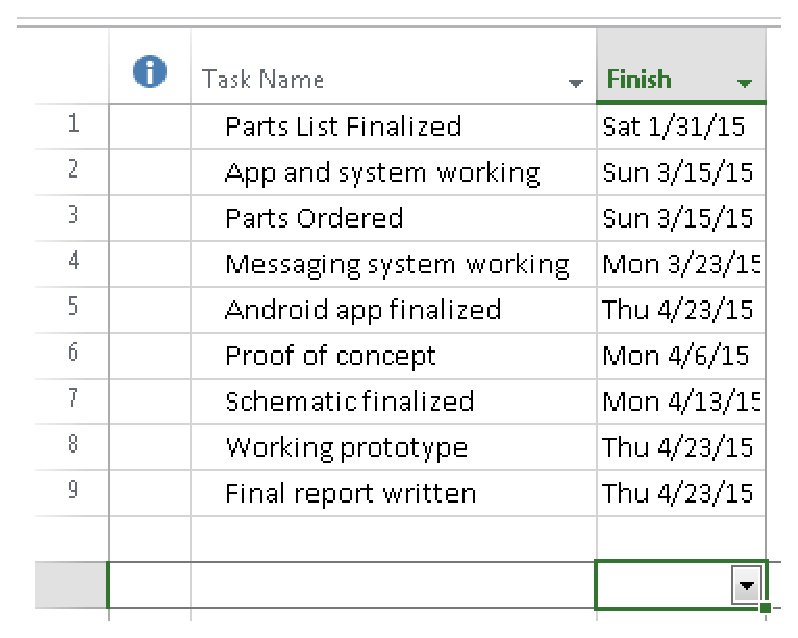
\includegraphics[width=0.8\textwidth]{schedule.eps} 
\caption{Final timeline} \label{schedule}
\end{figure}

\clearpage

\subsection*{Parts List}
% Table generated by Excel2LaTeX from sheet 'Sheet1'
\begin{table}[htbp]
  \centering
    \begin{tabular}{| c | c | c | c | c |}
    \hline
    Part  & Source & Unit Cost & Number  & Total \\
    \hline
    Raspberry Pi & Newark.com & \$40.00 & 1     & \$40.00 \\
	\hline    
    Arduino Uno & Sparkfun.com & \$29.95 & 1     & \$29.95 \\
    \hline
    Child Case & Amazon.com & \$13.71 & 1     & \$13.71 \\
	\hline
    USB Wifi Adapter & Amazon.com & \$8.99 & 1     & \$8.99 \\
	\hline
    Hub Case & Amazon.com & \$8.99 & 1     & \$8.99 \\
	\hline
    Power Cord & Amazon.com & \$5.99 & 1     & \$5.99 \\
	\hline
    Battery Case & Amazon.com & \$5.70 & 1     & \$5.70 \\
	\hline
    RF Rec & Sparkfun.com & \$4.95 & 1     & \$4.95 \\
	\hline
    RF Trans & Sparkfun.com & \$3.95 & 1     & \$3.95 \\
	\hline
	AA Battery & Amazon.com & \$0.43 & 6     & \$2.59 \\
	\hline
    IR Rec & Sparkfun.com & \$1.95 & 1     & \$1.95 \\
	\hline
	Voltage Regulator & Sparkfun.com & \$0.95 & 2     & \$1.90 \\
	\hline
    Battery Clip & Amazon.com & \$1.58 & 1     & \$1.58 \\
	\hline
	IR LED & Sparkfun.com & \$0.95 & 1     & \$0.95 \\
	\hline
    2N3904 & Mouser.com & \$0.41 & 2     & \$0.82 \\
	\hline
	 Switch & Amazon.com & \$0.75 & 1     & \$0.75 \\
	\hline
    Red LED & Sparkfun.com & \$0.35 & 2     & \$0.70 \\
	\hline
    Screw terminal & Amazon.com & \$0.21 & 3     & \$0.62 \\
    \hline
    $330 \Omega$ resistor & Mouser.com & \$0.10 & 5     & \$0.50 \\
	\hline
    Yellow LED & Sparkfun.com & \$0.35 & 1     & \$0.35 \\
	\hline
    $1 M\Omega$ resistor & Radioshack & \$0.25 & 1     & \$0.25 \\
	\hline
    0.1 uF cap & Sparkfun.com & \$0.25 & 1     & \$0.25 \\
	\hline
    Total &       &       &       & \$135.43 \\
    \hline
    \end{tabular}%
  \label{tab:parts}%
\end{table}%

\clearpage
\subsection*{Data Sheets}
\begin{itemize}
\item{RF Transmitter: \url{http://cdn.sparkfun.com/datasheets/Wireless/General/TWS-BS-6_315MHz_ASK_RF_Transmitter_Module_Data_Sheet.pdf}}
\item{RF Receiver: \url{http://www.dipmicro.com/store/RF315PAIR}}
\item{IR LED: \url{http://cdn.sparkfun.com/datasheets/Components/LED/YSL-R531FR1C-F1.pdf}}
\item{Colored LEDs: \url{http://www.sparkfun.com/datasheets/Components/LED/COM-09590-YSL-R531R3D-D2.pdf}}
\item{Voltage Regulators: \url{http://cdn.sparkfun.com/datasheets/Components/General/TO-220.pdf}}
\item{2N3904 BJT: \url{http://www.sparkfun.com/datasheets/Components/2N3904.pdf}}
\end{itemize}

\clearpage

\subsection*{Circuit Diagrams}
\begin{figure}[ht!]
\centering % must do this or your figure won't be centered
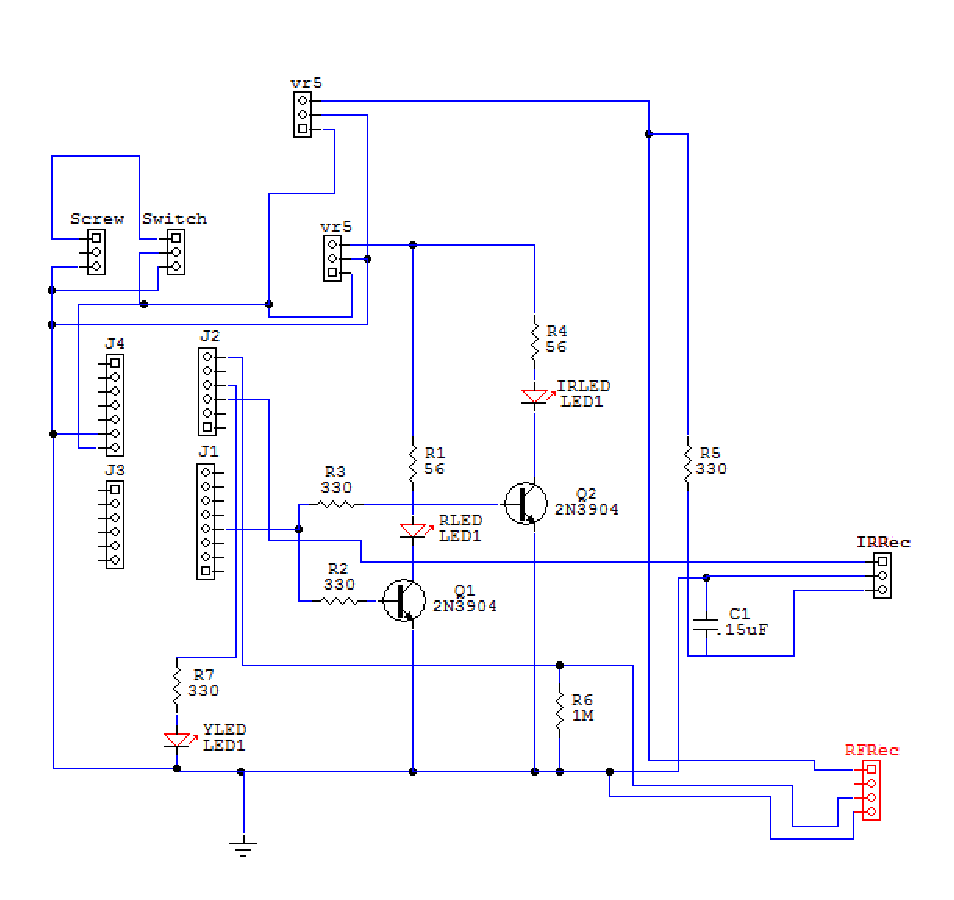
\includegraphics[width=0.8\textwidth]{CKT-child.eps} 
\caption{The circuit diagram for the \emph{child}.} \label{ckt-child}
\end{figure}

\begin{figure}[ht!]
\centering % must do this or your figure won't be centered
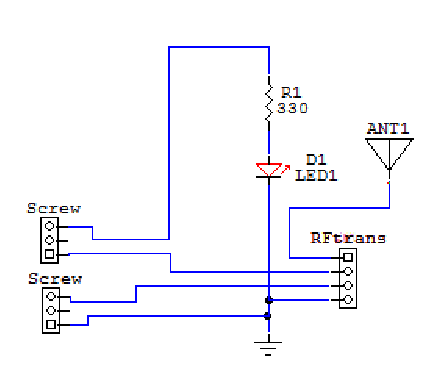
\includegraphics[width=0.8\textwidth]{CKT-hub.eps} 
\caption{The circuit diagram for the \emph{hub}.} \label{ckt-hub}
\end{figure}

\clearpage

\subsection*{Construction Diagrams}
\begin{figure}[ht!]
\centering % must do this or your figure won't be centered
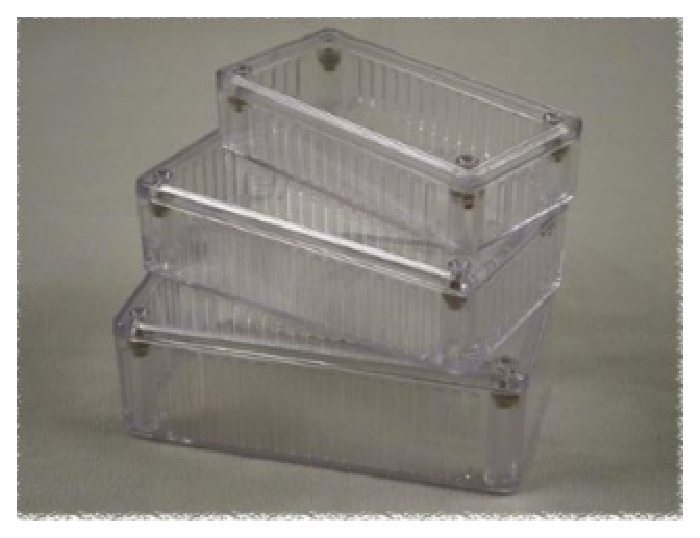
\includegraphics[width=0.5\textwidth]{child-packaging.eps} 
\caption{Child device packaging. \cite{hammond}} \label{child-pack}
\end{figure}

\begin{figure}[ht!]
\centering % must do this or your figure won't be centered
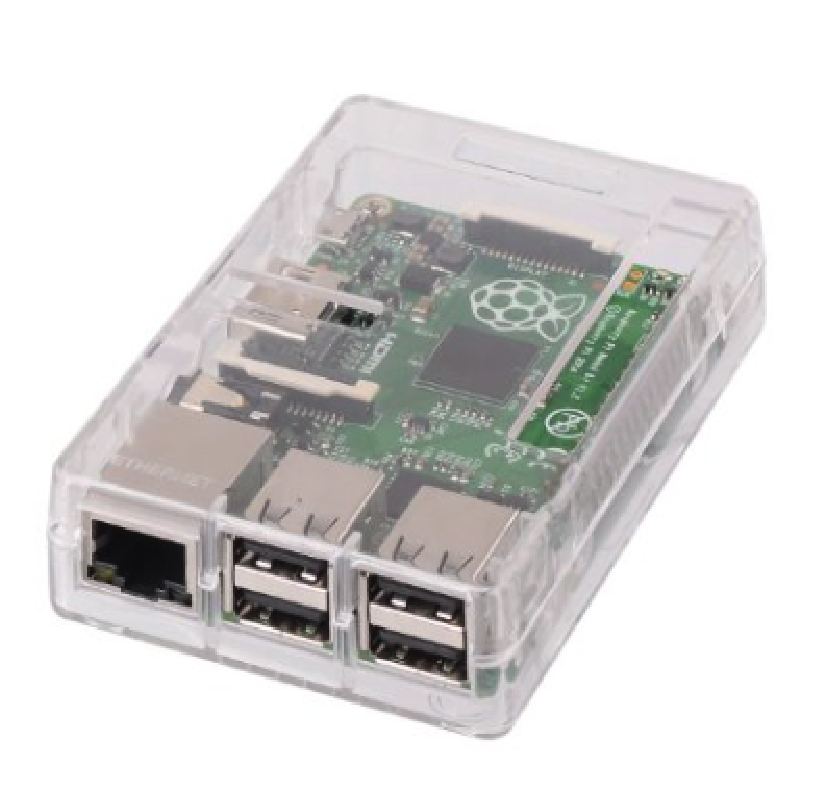
\includegraphics[width=0.5\textwidth]{hub-packaging.eps} 
\caption{Hub device packaging. \cite{kotek}} \label{hub-pack}
\end{figure}

\begin{figure}[ht!]
\centering % must do this or your figure won't be centered
\includegraphics[width=0.5\textwidth]{final.eps} 
\caption{Final packaging.} \label{final}
\end{figure}


\subsection*{Structure Charts for Code}
\begin{figure}[ht!]
\centering % must do this or your figure won't be centered
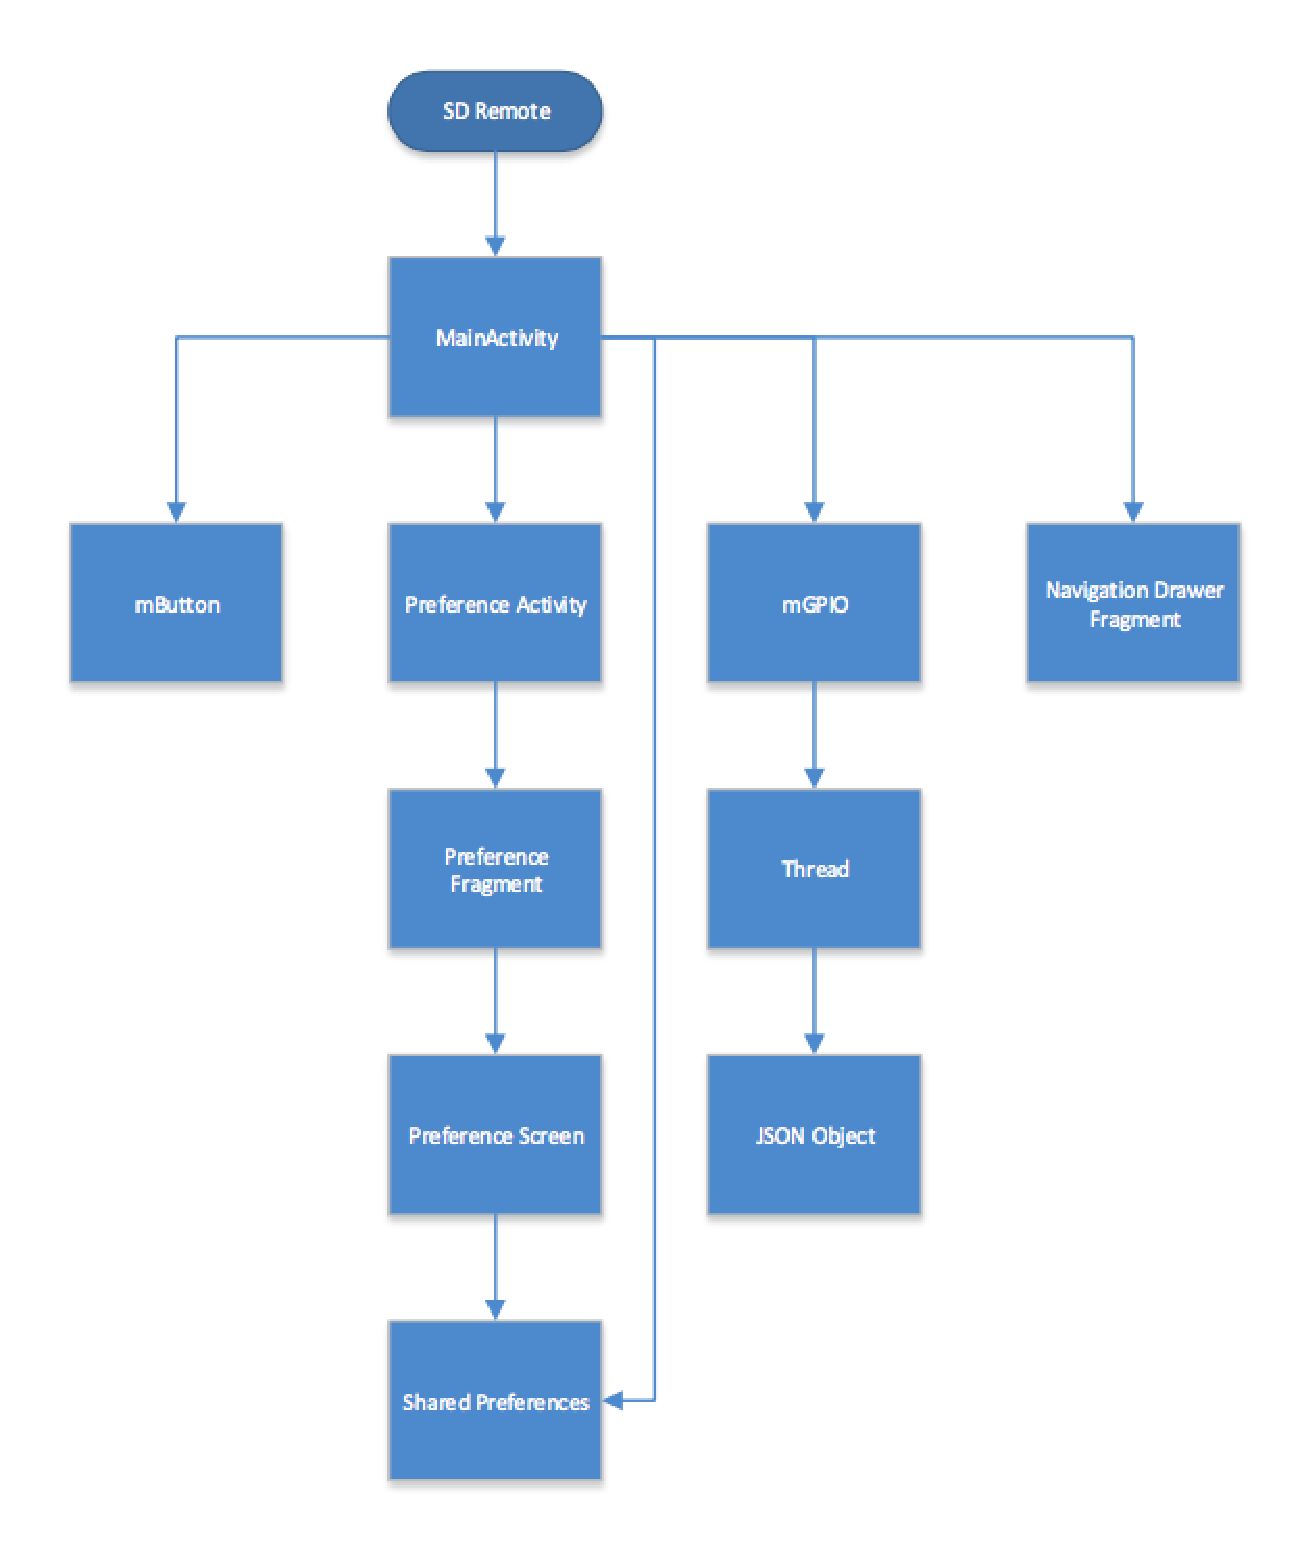
\includegraphics[width=0.8\textwidth]{SD-SDR.eps} 
\caption{The Structure Chart for the Android application.} \label{sd-sdr}
\end{figure}

\begin{figure}[ht!]
\centering % must do this or your figure won't be centered
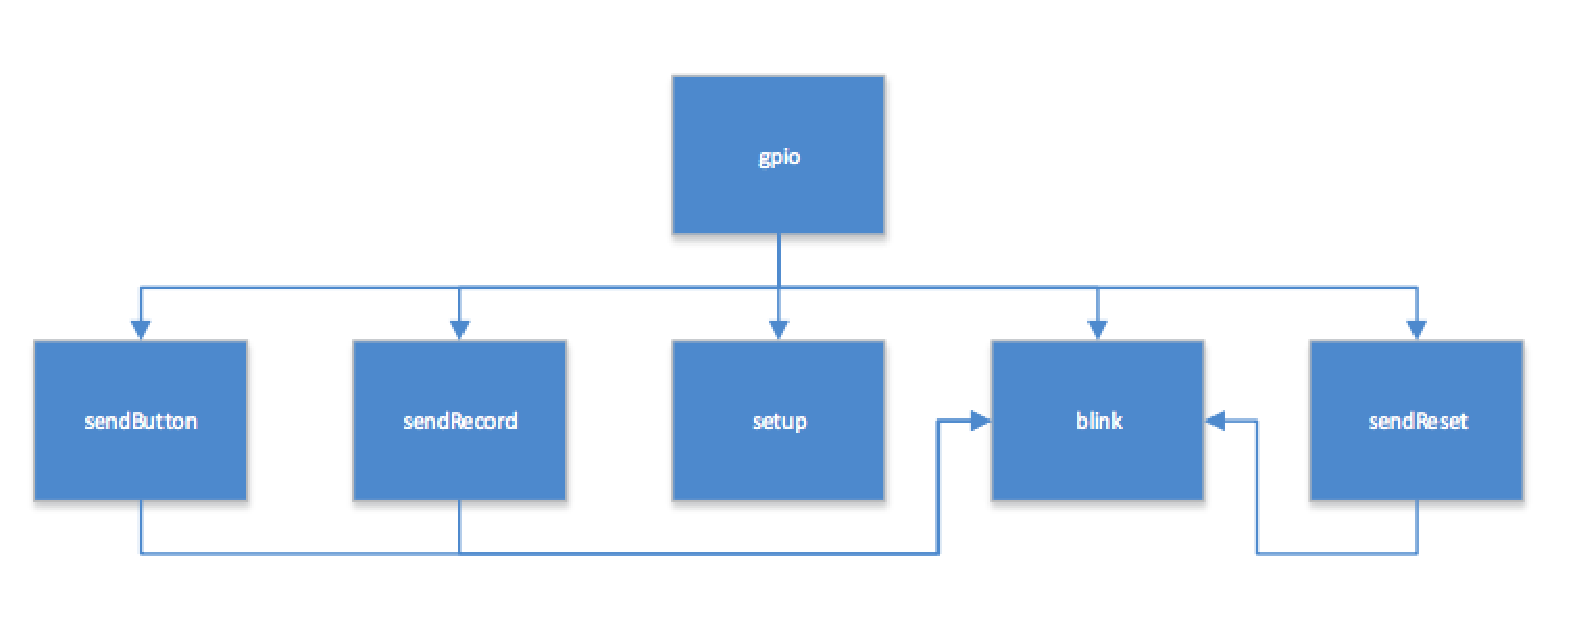
\includegraphics[width=0.7\textwidth]{SD-gpio.eps} 
\caption{The Structure Chart for \texttt{gpioV2.py}, which runs on the \emph{hub}.} \label{sd-gpio}
\end{figure}

\clearpage

\subsection*{UML Activity Diagrams for Code}
\begin{figure}[ht!]
\centering % must do this or your figure won't be centered
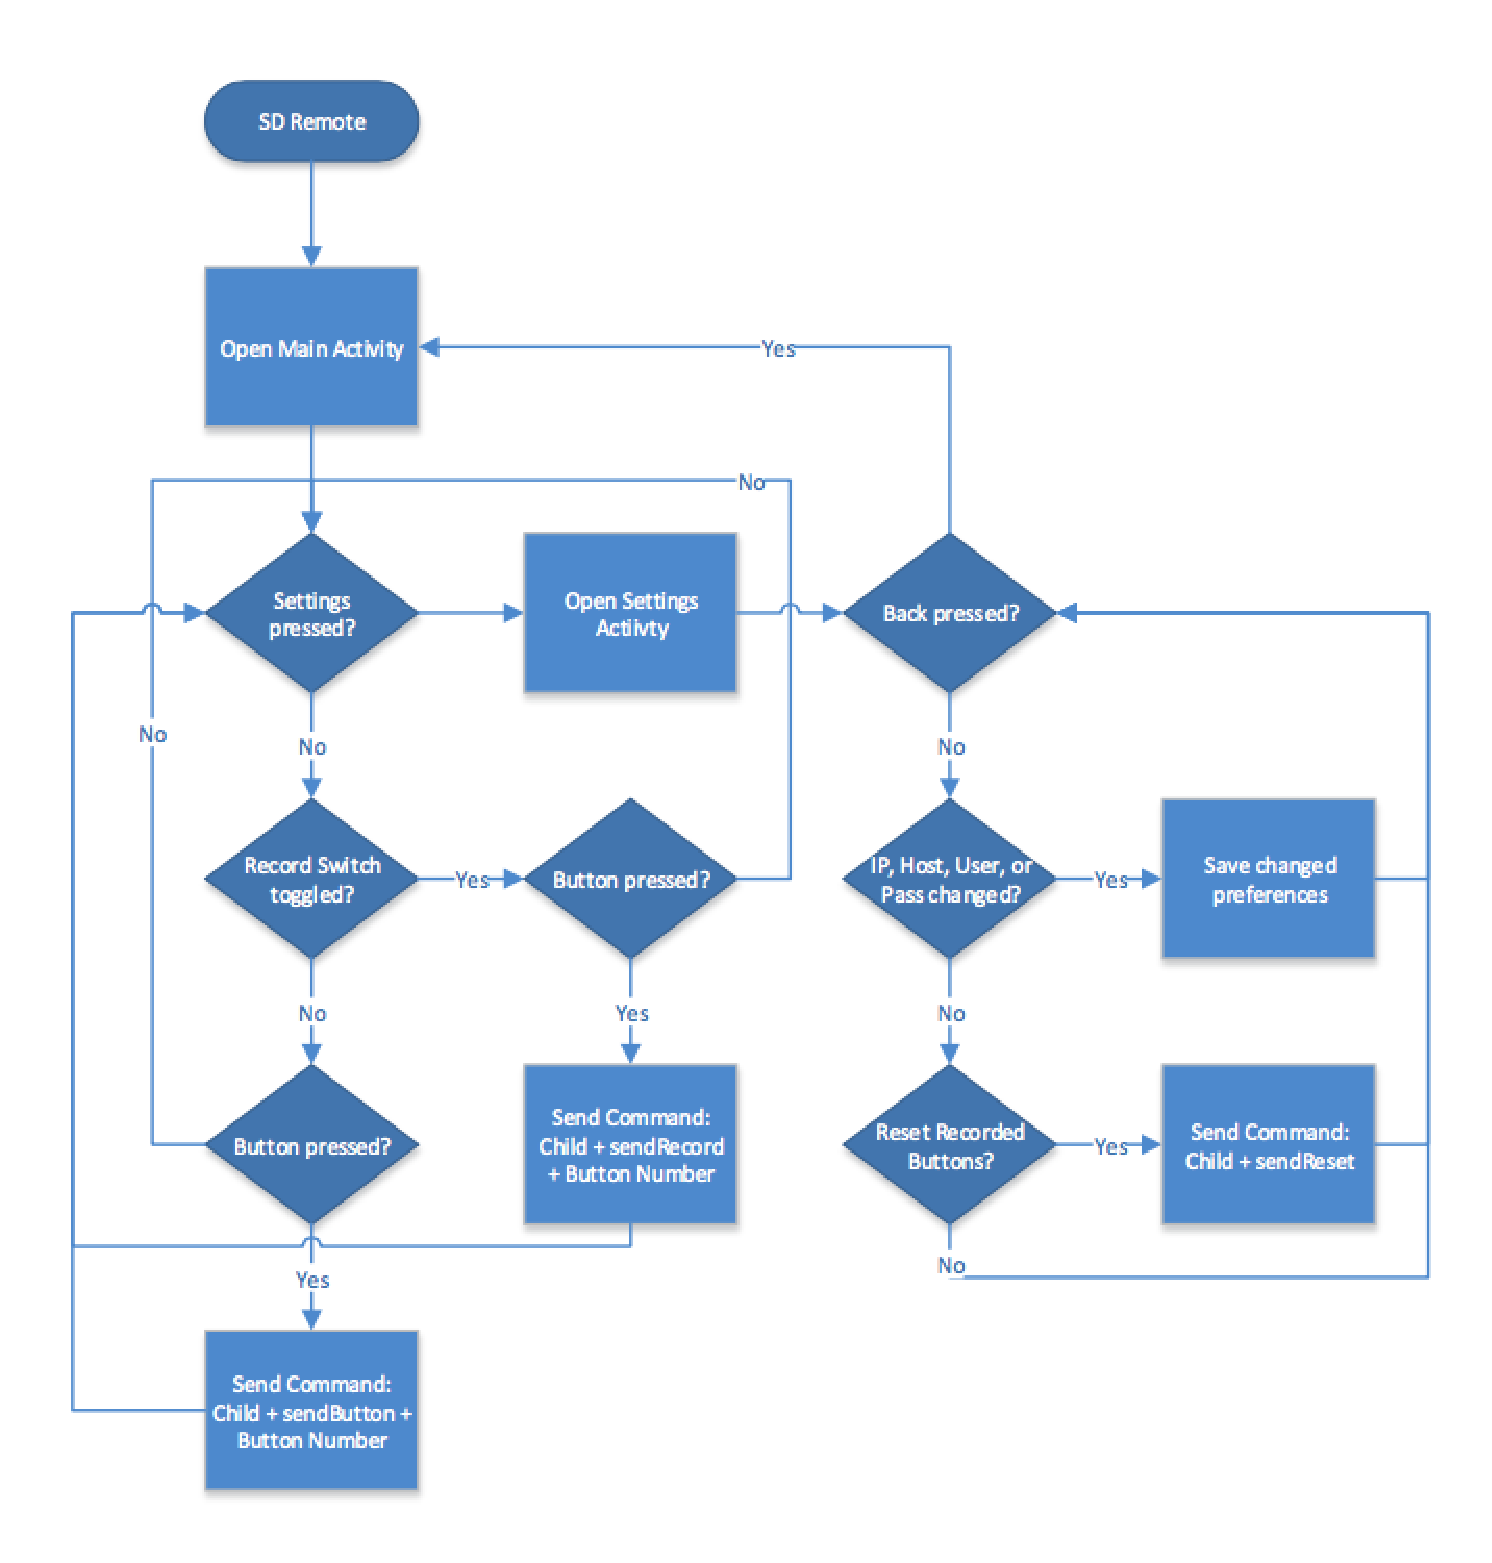
\includegraphics[width=0.8\textwidth]{AD-SDR.eps} 
\caption{The Activity Diagram for the Android application.} \label{ad-sdr}
\end{figure}

\begin{figure}[ht!]
\centering % must do this or your figure won't be centered
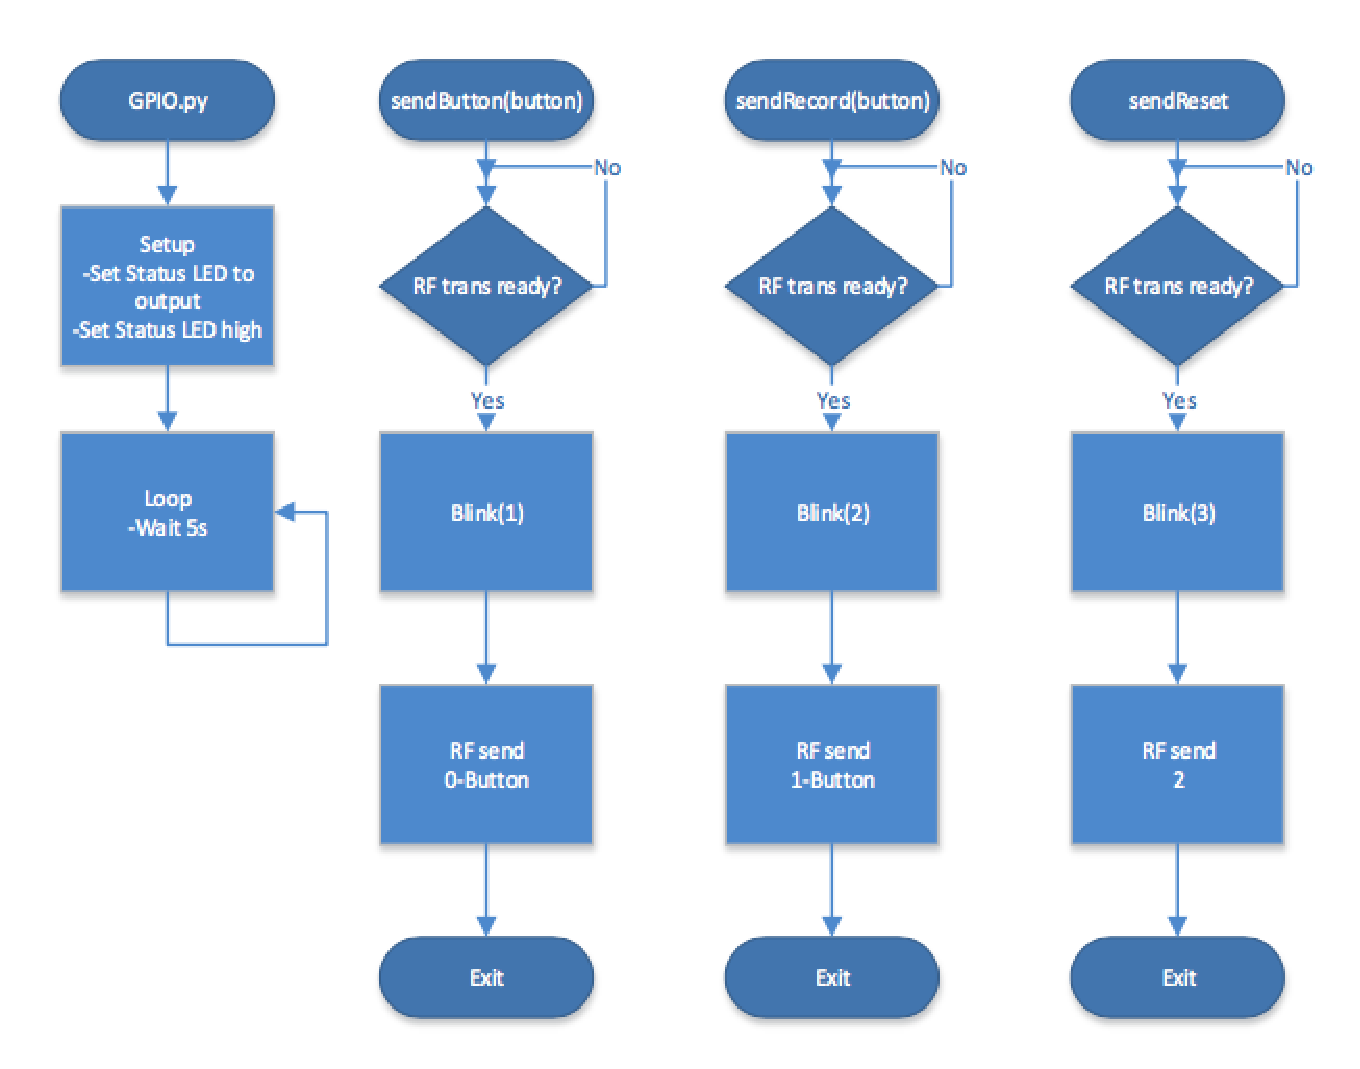
\includegraphics[width=0.8\textwidth]{AD-gpio.eps} 
\caption{The Activity Diagram for \texttt{gpioV2.py} on the \emph{hub}.} \label{ad-gpio}
\end{figure}

\begin{figure}[ht!]
\centering % must do this or your figure won't be centered
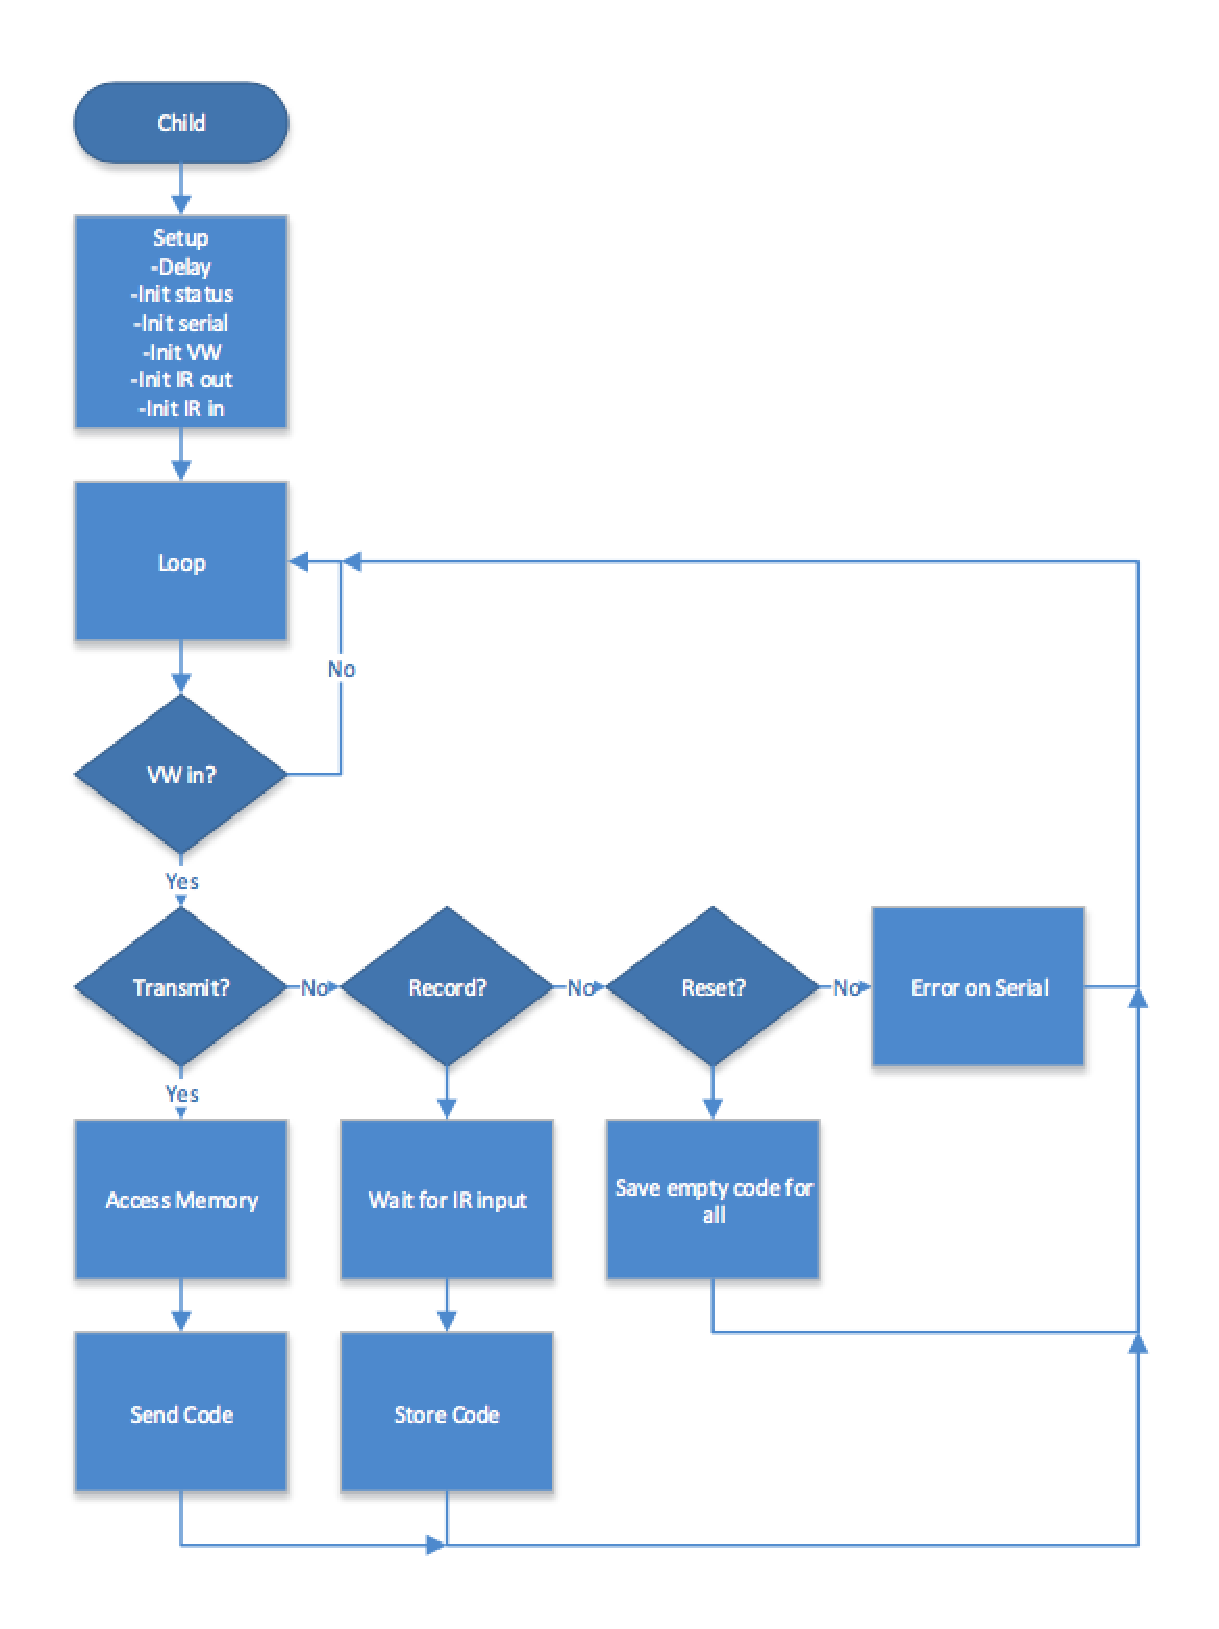
\includegraphics[width=0.8\textwidth]{AD-childuino.eps} 
\caption{The Activity Diagram for \texttt{childuino.ini} on the \emph{child}. } \label{ad-childuinio}
\end{figure}

\clearpage

\subsection*{Code}
\subsection{Android Application}
\lstinputlisting[caption={\texttt{AndroidManifest.xml}. This file is for the SDRemote application. It configures the application as required by Android.},label={code_manifest}]{AndroidManifest.xml} 

\lstinputlisting[caption={\texttt{MainActivity.java}. This class, which is equivalent to a main.cpp, contains most of the code for the Android application.}, label={code_main}]{MainActivity.java} 
 
\lstinputlisting[caption={\texttt{UserSettingsActivity.java}. This Activity displays settings when the ``Settings" button is pressed in the main application window. Some preferences are hidden from the user.},label={code_settings}]{UserSettingsActivity.java} 
 
\lstinputlisting[caption={\texttt{mGPIO.java}. This class takes care of sending commands from the Android application.},label={code_mgpio}]{mGPIO.java} 
 
\lstinputlisting[caption={\texttt{activity\_main.xml}. This file defines user interface elements of the main screen of the Android application.},label={code_mainact}]{activity_main.xml} 
 
\lstinputlisting[caption={\texttt{preferences.xml}. This file defines all of the Android application's preferences.},label={code_preferences}]{preferences.xml} 
 
\lstinputlisting[caption={\texttt{strings.xml}. This file defines Strings used in the Android application. They are defined here to make translating easier.},label={code_strings}]{strings.xml} 

\lstinputlisting[caption={\texttt{mButton.java}. This class creates an Android button that can also easily be toggled to unclickable and transparent.},label={code_button}, language={Java}]{mButton.java} 

\hfill \break
\subsection{Hub}

\lstinputlisting[caption={\texttt{gpioV2.py}. This is a Python script for starting an HTTP server and listening for commands.}, language=Python, label={code_gpio}]{gpioV2.py}

\hfill \break
\subsection{Child}

\lstinputlisting[caption={\texttt{childuino.ino}. The program responsible for controlling the \emph{child} device.},language={C++}, label={code_childuino}]{childuino.cpp} 
 
\end{document}